% HEV Energy Management Strategy (EMS) progress timeline
% Wide layout: year on the horizontal axis, capability tier on the vertical axis.
% Tune width/height with the x= and y= scales in the tikzpicture options.
\documentclass[tikz,border=6pt]{standalone}
\usepackage{tikz}
\usetikzlibrary{arrows.meta}

\begin{document}
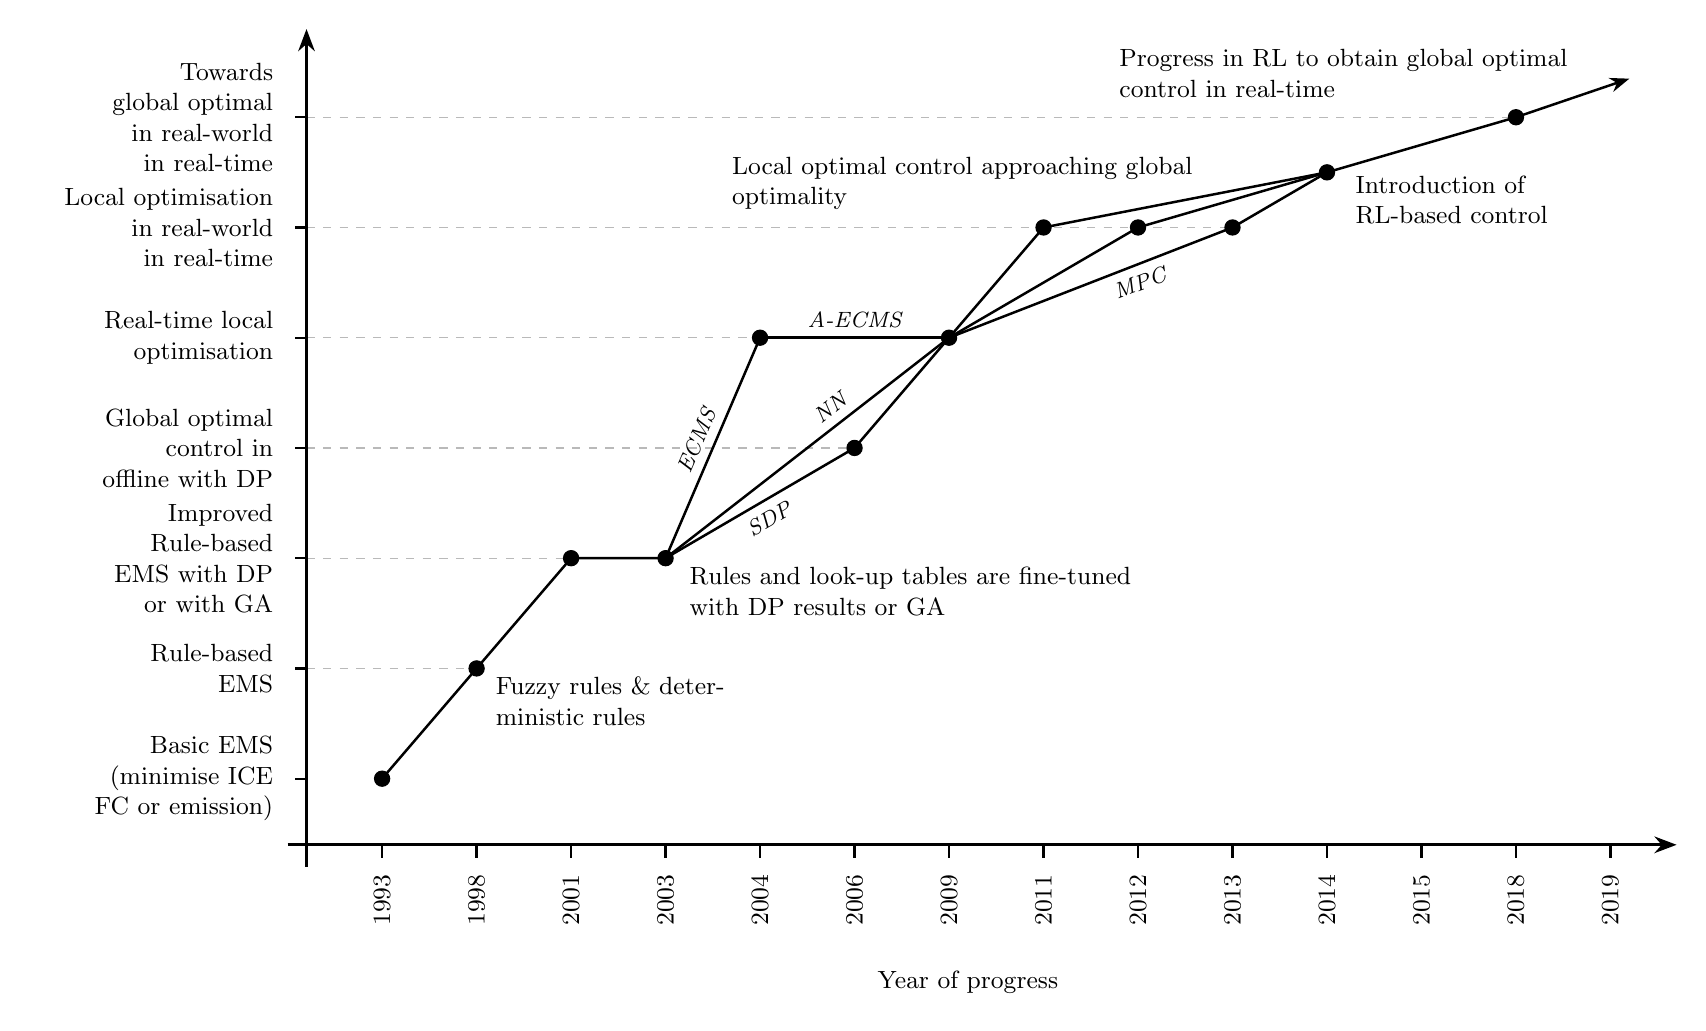
\begin{tikzpicture}[
    x=1.2cm, y=1.4cm,                       % <- widen: raise x= ; flatten: lower y=
    milestone/.style={circle, draw=black, fill=black, inner sep=0pt, minimum size=5.5pt},
    branch/.style={font=\footnotesize\itshape},
    annot/.style={font=\small, align=left, text width=3.2cm},
    tierlbl/.style={font=\small, align=right, text width=3.0cm, anchor=east},
    guide/.style={gray!55, dashed, line width=0.4pt},
    conn/.style={line width=0.9pt, line cap=round},
  ]

  % ---------- milestone coordinates (x = year slot, y = capability tier) ----------
  \coordinate (p1993) at (0.8,0.6);
  \coordinate (p1998) at (1.8,1.6);
  \coordinate (p2001) at (2.8,2.6);
  \coordinate (p2003) at (3.8,2.6);
  \coordinate (p2004) at (4.8,4.6);
  \coordinate (p2006) at (5.8,3.6);
  \coordinate (p2009) at (6.8,4.6);
  \coordinate (p2011) at (7.8,5.6);
  \coordinate (p2012) at (8.8,5.6);
  \coordinate (p2013) at (9.8,5.6);
  \coordinate (p2014) at (10.8,6.1);   % RL-based: between tier 6 and 7
  \coordinate (p2018) at (12.8,6.6);

  % ---------- dashed tier leaders ----------
  \draw[guide] (0,1.6) -- (p1998);
  \draw[guide] (0,2.6) -- (p2003);
  \draw[guide] (0,3.6) -- (p2006);
  \draw[guide] (0,4.6) -- (p2009);
  \draw[guide] (0,5.6) -- (p2013);
  \draw[guide] (0,6.6) -- (p2018);

  % ---------- connectors ----------
  \draw[conn] (p1993) -- (p1998) -- (p2001) -- (p2003);                 % backbone staircase
  \draw[conn] (p2003) -- (p2004) node[branch,midway,sloped,above] {ECMS};
  \draw[conn] (p2003) -- (p2009) node[branch,pos=0.62,sloped,above] {NN};
  \draw[conn] (p2003) -- (p2006) node[branch,pos=0.5,sloped,below] {SDP};
  \draw[conn] (p2006) -- (p2009);
  \draw[conn] (p2004) -- (p2009) node[branch,midway,sloped,above] {A-ECMS};
  \draw[conn] (p2009) -- (p2011);                                       % MPC fan-out
  \draw[conn] (p2009) -- (p2012);
  \draw[conn] (p2009) -- (p2013) node[branch,pos=0.65,sloped,below] {MPC};
  \draw[conn] (p2011) -- (p2014);                                       % converge into RL-based
  \draw[conn] (p2012) -- (p2014);
  \draw[conn] (p2013) -- (p2014);
  \draw[conn] (p2014) -- (p2018);                                       % RL progress
  \draw[conn,-{Stealth[length=7pt]}] (p2018) -- (14.0,6.95);            % trend arrow

  % ---------- milestone dots (drawn last, on top of lines) ----------
  \foreach \p in {p1993,p1998,p2001,p2003,p2004,p2006,p2009,p2011,p2012,p2013,p2014,p2018}
  \node[milestone] at (\p) {};

  % ---------- axes ----------
  \draw[-{Stealth[length=8pt]}, line width=1pt] (-0.2,0) -- (14.5,0);
  \draw[-{Stealth[length=8pt]}, line width=1pt] (0,-0.2) -- (0,7.4);

  % ---------- y-axis tier ticks + labels ----------
  \foreach \y/\txt in {%
    0.6/{Basic EMS\\(minimise ICE\\FC or emission)},
    1.6/{Rule-based\\EMS},
    2.6/{Improved Rule-based\\EMS with DP\\or with GA},
    3.6/{Global optimal\\control in\\offline with DP},
    4.6/{Real-time local\\optimisation},
    5.6/{Local optimisation\\in real-world\\in real-time},
  6.6/{Towards global optimal\\in real-world\\in real-time}}{%
    \draw[line width=0.8pt] (0,\y) -- (-0.12,\y);
    \node[tierlbl] at (-0.25,\y) {\txt};
  }

  % ---------- x-axis year ticks + labels (2015 & 2019 are bare ticks) ----------
  \foreach \x/\yr in {%
    0.8/1993, 1.8/1998, 2.8/2001, 3.8/2003, 4.8/2004, 5.8/2006,
    6.8/2009, 7.8/2011, 8.8/2012, 9.8/2013, 10.8/2014, 11.8/2015,
  12.8/2018, 13.8/2019}{%
    \draw[line width=0.8pt] (\x,0) -- (\x,-0.12);
    \node[font=\small, rotate=90, anchor=east] at (\x,-0.18) {\yr};
  }
  \node[font=\small] at (7.0,-1.25) {Year of progress};

  % ---------- prose annotations ----------
  \node[annot,anchor=west,text width=3.0cm] at (1.9,1.3)
  {Fuzzy rules \& deterministic rules};
  \node[annot,anchor=west, text width=6cm] at (3.95,2.3)
  {Rules and look-up tables are fine-tuned with DP results or GA};
  \node[annot,anchor=west,text width=6cm] at (4.4,6)
  {Local optimal control approaching global optimality};
  \node[annot,anchor=west,text width=2.8cm] at (11.0,5.85)
  {Introduction of RL-based control};
  \node[annot,anchor=west,text width=6cm] at (8.5,7.0)
  {Progress in RL to obtain global optimal control in real-time};

\end{tikzpicture}
\end{document}
